\documentclass[../main/main.tex]{subfiles}

\newdate{date}{10}{12}{2020}


\begin{document}

\marginpar{ \textbf{Lecture 21.} \\  \displaydate{date}. \\ Compiled:  \today.}

In general the \textbf{posterior distribution} is \textit{difficult} to obtain analytically, therefore \textbf{numerical integration} is required.

\section{Monte Carlo approaches}

In order to \textbf{compute the likelihood} as a starting point, if our knowledge is none, we can use a \textbf{grid of points} in order to compute $p(\vec{\theta}|y)$ for $\theta_1,\theta_2,...\theta_n$ equally spaced. In this way, we \textit{approximate} the continuous density function $p(\vec{\theta}|y)$ with the \textbf{discrete density function}:
\begin{equation*}
   \frac{p(\theta_i |y)} {\sum_i p(\theta_i|y)}
\end{equation*}
However, this approach is to become rapidly \textit{unfeasibile} as the dimensionality of the parameter space becomes larger.

Another approximation one might want to take is the \textbf{Trapezoidal approximation}: after computing $p(\theta|y)$ for a discrete set of points $\theta_1,...\theta_n$ we can approximate $p(\theta|y)$ with a piecewise-linear function, connecting the $p(\theta_i|y)$ points with linear segments.


One may ask now how to \textbf{numerically sample} $p(\theta|y)$. In order to do so, we use a \textit{positive function} $g(\theta)$ defined for all $\theta$ such that $p(\theta|y) > 0$. Moreover it must hold that:
\begin{itemize}
\item we are able to draw samples from $g(\theta)$;
\item for some \textit{constant} $M$ the ratio $p(\theta|y)/g(\theta) \leqslant M$ is defined;
\item $g(\theta)$ must have a finite integral.
\end{itemize}
The \textbf{rejection sampling} algorithm hence is constituted by these two steps (Fig. \ref{fig:21_01}):
\begin{itemize}
    \item  sampling $\theta$ at random from the pdf of $g(\theta)$;
    \item with probability that is given by the ratio $p(\theta|y)/Mg(\theta)$ we accept $\theta$ pretending it is drawn from the real $p(\theta|y)$ we wanted to approximate.
\end{itemize}


\begin{figure}[h!]
\centering
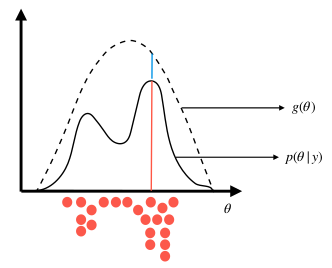
\includegraphics[width=0.45\textwidth]{../lessons/image/21/image01.png}
\caption{\label{fig:21_01} Rejection sampling method in order to sample from a distribution}
\end{figure}

The choice $g(\theta)$ plays an important role, specially wrt computational effort: the more different it is from $p(\theta|y)$, the higher is the rejection rate. However, if we have no information about the shape of $p(\theta|y)$ we should use a flat $g(\theta)$ (see Fig. \ref{fig:21_02a}). On the other hand using the \textit{trapezoidal approximation} to define $g(\theta)$ we can reduce this problem (see Fig. \ref{fig:21_02b}).

\begin{figure}[h!]
\begin{minipage}[c]{0.5\linewidth}
\subfloat[][Rejection sampling using a "box" distribution. Efficiency is very low.]{ 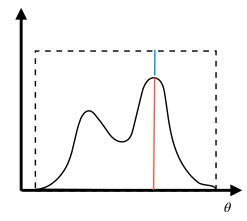
\includegraphics[width=0.8\textwidth]{../lessons/image/21/image02a.png}  \label{fig:21_02a} }
\end{minipage}
\begin{minipage}[]{0.5\linewidth}
\centering
\subfloat[][Rejection sampling using $g(\theta)$ as a trapezoidal approximation for $p(\theta|y)$. Indeed we reach a high efficiency.]{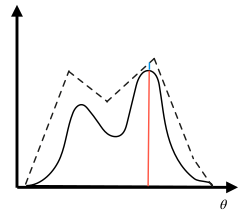
\includegraphics[width=0.8\textwidth]{../lessons/image/21/image02b.png}  \label{fig:21_02b} }
\end{minipage}
\caption{\label{fig:}}
\end{figure}

We will now introduce the most efficient way to sample from distribution: \textbf{Markov Chain Monte Carlo} (MCMC). The general idea behind them is to start from an initial point in the parameter space $\theta_0$, and starting from it to create a \textit{random walk}. It is a \textit{sequence} $\theta_0, \theta_1,...\theta_t$ where each $\theta_i$ is draw from a given \textit{transition distribution}, built such that the random walk converges to $p(\theta|y)$. That is to say we need to run the simulation long enough such that the distribution of the current draws becomes close enough to the stationary distribution $p(\theta|y)$.
An example of MCMC is the so called \textbf{Metropolis algorithm} (see Fig. \ref{fig:21_03a}, \ref{fig:21_03b}). As in the general case we draw samples from a starting point $\theta_0$ and then we iterate the following procedure for $t = 1, 2...$:
\begin{itemize}
    \item sample a candidate point $\theta^*$ from a jumping distribution $J_t(\theta^*|\theta^{t-1})$. This distribution \textit{must} be \textbf{symmetric}, i.e. such that $J_t(\theta_a|\theta_b) = J_t(\theta_b|\theta_a) \quad \forall a,b,t$;
    \item compute the ratio of the densities:
    \begin{equation*}
    r = \frac{p(\theta^*|y)}{p(\theta^{t-1}|y)}
    \end{equation*}
    \item update $\theta^t = \theta^*$ with probability $\text{min}(r,1)$ (Fig. \ref{fig:21_03b}), otherwise $\theta^* = \theta^{t-1}$ (Fig. \ref{fig:21_03a}).
\end{itemize}

\begin{figure}[h!]
\begin{minipage}[c]{0.5\linewidth}
\subfloat[][If we jump from a less probable $\theta$ for to a more probable one, we \textit{always accept} the drawn candidate $\theta^*$. ]{ 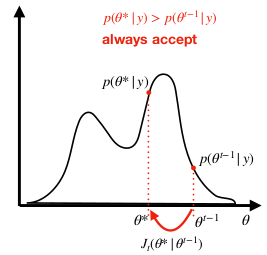
\includegraphics[width=0.8\textwidth]{../lessons/image/21/image03a.png}  \label{fig:21_03a} }
\end{minipage}
\begin{minipage}[]{0.5\linewidth}
\centering
\subfloat[][If we jump from a more probable $\theta$ for $p(\theta)$ to a less probable one, we \textit{sometimes accept} the move according to a probability given by the ratio between the candidate $p(\theta^*|y)$ and $p(\theta^{t-1}|y)$. ]{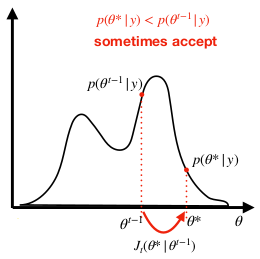
\includegraphics[width=0.8\textwidth]{../lessons/image/21/image03b.png}  \label{fig:21_03b} }
\end{minipage}
\caption{\label{fig:} Metropolis Algorithm.}
\end{figure}


Note that it is possible to show that for a \textit{Metropolis Algorithm}, the Markov chain converges to a stationary distribution, which is $p(\theta|y)$. One may want to apply what we discussed so far and simulate \textit{multiple chains} simultaneously with starting points dispersed in the parameter space.
We keep monitoring the quantity (i.e. the parameter) of our interest and measuring variation between and within the different sequences, until all of them \textbf{converge} to a \textbf{unique distribution}. Therefore, the initial part of the random walk has to be neglected since samples are strongly correlated, we refer to this fact as \textbf{burn-in}.

Let us now consider the following example: we want to sample from a posterior density that is a \textbf{bivariate unit normal}. The probability density function is therefore:
\begin{equation*}
    p(\theta_1, \theta_2 |y) = \mathcal{N}(\theta_1, \theta_2|0,\mathbb{1}_2) = \frac{1}{2\pi} e^{- \frac{\theta_1^2+\theta_2^2}{2}}
\end{equation*}
where $\mathbb{1}_2$ is the $2\times 2$ identity matrix.

As for the \textbf{jumping distribution} of the kind $J_t(\theta^*|\theta^{t-1}) = \mathcal{N}(\theta^*|\theta^{t-1}, \sigma^2\mathbb{1}_1 )$, that we recall \textit{must} be \textbf{symmetric}, we can choose a \textit{bivariate normal} as well:
\begin{equation*}
    J(\theta^*_1,\theta^*_2| \theta^{t-1}_1,\theta^{t-1}_2) = \frac{1}{2\pi \sigma^2}e^{-\frac{(\theta_1^* - \theta_1^{t-1} )^2+(\theta_2^* - \theta_2^{t-1})^2}{2 \sigma^2}}
\end{equation*}
The only \textbf{parameter} we need to tune as for the \textit{jumping distribution} is $\sigma$:
\begin{itemize}
    \item \textbf{large} $\sigma$: the larger it is, the larger jumps will be allowed such that we will be able to explore a larger space of parameters. On the other hand, almost all proposal will be rejected. Hence, despite the large inefficiency, we will end up being stuck;
    \item \textbf{small} $\sigma$: the chain will be too slow and the algorithm will be inefficient;
    \item \textbf{best} $\sigma$: we use as a \textit{rule of thumb} a condition over the \textit{acceptance rate} that has to be in the interval $0.23-0.44$.
\end{itemize}

\begin{figure}[h!]
\centering
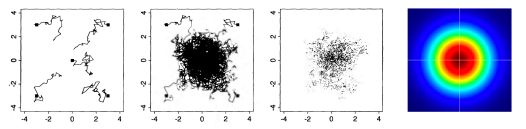
\includegraphics[width=0.90\textwidth]{../lessons/image/21/image04.png}
\caption{\label{fig:21_04} Markov Chain Monte Carlo at different stages of simulation. The distribution we use to sample from are bivariate Gaussians.}
\end{figure}














\chapter{Outbreak Analysis}

Let us apply all the knowledge we have acquired so far to a real world problem. We want to understand what we need to do when we observe an \textbf{outbreak} of an \textbf{emerging pathogen} about which we know \textit{nothing}. Let us immerse ourselves in the following situation: to us all epidemiological characteristic, namely $\mu,\beta$, generation time, are unknown. We will use COVID-19 as a \textit{paradigmatic} case. For Fig. \ref{fig:21_05} one can tell that we achieved very good results in studying the disease as fast as possible: indeed all relevant quantities were computed in a couple of months.

\begin{figure}[h!]
\centering
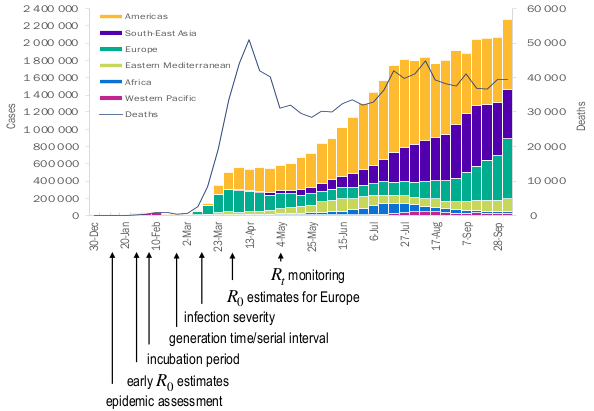
\includegraphics[width=0.90\textwidth]{../lessons/image/21/image05.png}
\caption{\label{fig:21_05} \textbf{COVID-19 outbreak analysis}
Number of COVID-19 cases reported weekly by WHO Region, and global deaths, 30 December 2019. Arrows describe the moment at which the quantity reported has been computed. The epidemic assessment started from the letter written by Imperial College.}
\end{figure}

\section{Basic Reproductive Ratio $\pmb{R_0}$ estimation}

We will discuss now how to \textbf{process} the raw data in order to obtain, for instance, the \textbf{basic reproductive ratio} $R_0$. It is a really relevant quantity since we can retrieve the \textit{final attack rate} if the virus spread: this is helpful in policy making to understand how much serious the disease can be, as well as how far we are from the epidemic threshold and how many infections/deaths we might expect. 

\subsection{$\pmb{R_0}$ from the early exponential growth}

We will try to obtain $R_0$ using the \textit{early exponential growth} typical of epidemic spread. This is indeed useful for \textbf{real time analyses} of highly transmissible infections (i.e. you see an exponential growth of cases).

The estimate of $R_0$ will therefore computed by the means of the \textbf{exponential growth}, and obviously it is valid in the case we observe an epidemic. We will start to tackle this problem first introducing a simple version of the \textit{Kermack and the McKendrick model}\footnote{The Kermack-McKendrick model is an SIR model for the number of people infected with a contagious illness in a closed population over time. It also assumes a completely homogeneous population with no age, spatial, or social structure.} according to which the \textbf{incidence} at the \textbf{early stages is} (Fig. \ref{fig:21_06a} ):
\begin{equation}
    I(t) = I_0 e^{Gt} = I_0 e^{\mu(R_0-1)t}
\end{equation}
We must observe indeed a region where cases grow exponentially: here we fit using the curve just introduced. Reverting this last formula we are able to \textbf{estimate} $R_0$ from the \textit{exponential growth factor} $G$:
\begin{equation}
    R_0 = \mu^{-1} G + 1
\end{equation}
In this way we are \textbf{implicitly assuming} that \textit{infectivity} $\beta$ remains constant for the whole period of infection. It is indeed a strong, as well as unrealistic, assumption. Moreover, we assume that \textit{recovery} is a Poisson process, whose waiting times are exponentially distributed with average $\mu^{-1}$.


\begin{figure}[h!]
\begin{minipage}[c]{0.5\linewidth}
\subfloat[][Exponential early growth for SIR model.]{ 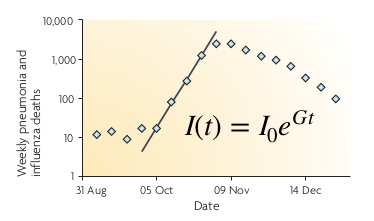
\includegraphics[width=0.8\textwidth]{../lessons/image/21/image06a.png}  \label{fig:21_06a} }
\end{minipage}
\begin{minipage}[]{0.5\linewidth}
\centering
\subfloat[][More general distribution for infectiousness, which might vary on time.]{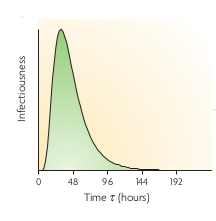
\includegraphics[width=0.8\textwidth]{../lessons/image/21/image06b.png}  \label{fig:21_06b} }
\end{minipage}
\caption{\label{fig:21_06}}
\end{figure}


We define the \textbf{Generation time} $T_c$ as the average time from infection of the infector to the infection of the infected. In this case, it holds that the average generation time is the average infectious duration $T_c = \mu^{-1}$, hence we can rewrite:
\begin{equation}
    R_0 = T_c G + 1
\end{equation}
However, this means that \textbf{infectious periods} are \textbf{exponentially distributed}, which is quite \textit{unrealistic}\footnote{Wallinga, Lipsitch, How generation intervals shape the relationship between growth rates and reproductive numbers Proc. R. Soc B (2007) 274, 599}. Another \textit{unrealistic} aspect is the \textbf{lack} of \textbf{exposed period}, which is quite always present.

Let us consider the more general situation as possible where the \textit{generation times} distribution is $w(\tau)$. We recall now that the \textbf{transmissibility generic function} $\beta(\tau)$ can be rewritten as function of the generating time as:
\begin{equation}
    w(\tau) = \frac{\beta(\tau)}{R_0}
    \label{eqn:w(tau)}
\end{equation}
This means that there is a period in which we are more likely to infect someone once infected, i.e. we are more infectious. Obviously, this is the peak in the distribution $w(\tau)$ (see Fig. \ref{fig:21_06b}).  The other way around to see it is the following: the time needed in order to generate a secondary case, which might be in number more than one, distributes as in Fig. \ref{fig:21_06b}.

Let us imagine to have a number $I(u)$ of newly infected individuals at time $u$. The \textbf{number of individuals they will infect} at time $t = u + \tau$ in a time interval $\delta \tau$ is a random process, and follows a \textbf{Poisson} distribution with mean:
\begin{equation}
    I(u) \beta (\tau) \delta \tau = I(t-\tau) \beta (\tau) \delta \tau
\end{equation}
One can easily see that the number of \textbf{newly generated} infected people \textit{does} depend on the number of \textit{previously infected} individuals. Formally, this is a \textbf{renewal equation} (Lotka-Euler equation)\footnote{a.k.a., borrowed from population dynamics. New births depend on people that were born 20-30 years ago: for instance their number (larger it is, the more births we expect), fecundity rate and how this parameter evolves during the whole lifespan of a person. Many models from ecology and demography can be applied to the epidemiological framework.}:
\begin{equation}
    I(t) = \int_0^\infty I(t - \tau) \beta(\tau) d \tau
\end{equation}
Simple $SIR$ model actually accounts for these last considerations, but it assumes that generation times distribution is exponential. We wanted to drop this assumption: we are indeed considering non-markovian epidemics. For this reason we had to introduce the aforementioned \textbf{integral equation}, which takes into account the exponential case too, and we could not write an exponential equation any more. Only for now, we are assuming well-mixed and therefore infinite population.

We want now to use the \textit{renewal equation} in order to estimate $R_0$. This can be done however \textit{only} when we observe an \textbf{exponential growth} of cases, according to which we can derive the \textit{exponential growing factor} $G$. Hence we can write the infectious people at time $I(t)$ in function of infectious people at time $t-\tau$ as follows:
\begin{equation}
    I(t) = I(t-\tau) e^{G\tau}
\end{equation}
By using last equality, the renewal equation becomes:
\begin{equation}
    I(t) = \int_0^\infty I(t) e^{-G \tau } \beta(\tau) d\tau
\end{equation}
Dividing both sides by $I(t)$ and replacing  \ref{eqn:w(tau)} in the last equation, we end up with:
\begin{equation}
    \frac{1}{R_0} = \int_0^\infty e^{-G \tau} w(\tau) d \tau
\end{equation}
From which we can provide an estimate for $R_0$. One should have noted that it is the \textbf{Laplace Transform} of $w(\tau)$: therefore we are able to relate directly $R_0$ to the generation times $w(\tau)$ distribution, specially to its moments generating function via $\mathcal{M}(z) = \int_0^\infty e^{z \tau} w(\tau) d\tau$:
\begin{equation}
     R_0 = \frac{1}{\mathcal{M}(-G)}
\end{equation}
We recall now the \textbf{properties} of the \textit{Laplace Transform} and its \textbf{epidemiological implications}:
\begin{itemize}
\item $\mathcal{M}_{w(\tau)}(z) \geqslant 0 \implies R_0 \geqslant 0$ because the Laplace transform is \textit{always} greater or equal than zero.
\item $\mathcal{M}_{w(\tau)}'(z) = \int_0^\infty \tau e^{z \tau} w(\tau)d\tau >0 \implies R_0$ is an increasing function of $G$, since the derivative of the Laplace transform is always greater than zero. Bigger the exponential growth, bigger is $R_0$.
\item $\mathcal{M}_{w(\tau)}(0) = \int_0^\infty w(\tau) d\tau = 1 \implies \ \text{if} \ G=0 \implies R_0 = 1$ from normalization condition. If we observe a flat curve, i.e. no exponential growth, then $R_0 = 1$.
\end{itemize}

Let us assume that $w(\tau)$ is distributed as a Gaussian, that we recall is the least informative distribution\footnote{It means that we know only the mean $\mu$ and the variance $\sigma^2$ of a distribution and nothing more.}. We know from theory that its \textit{Laplace Transform} is:
\begin{equation*}
    w(\tau) = \mathcal{N}(T_c, \sigma^2) \implies R_0 = e^{GT_c - (1/2)G^2\sigma^2}
\end{equation*}
This means that $R_0$ depends also on the variance of generation times distribution. Let is assume that the generation time is like the infectious period ($\expval{T_c} \sim \mu^{-1}$). For a given $\expval{T_c}$, if the variability  $\sigma^2$ of the generation times is higher, then the exponential term becomes lower, hence leading to lower $R_0$ (see Fig. \ref{fig:21_07}). For instance: if an individual remains infected for a shorter period, it is going to produce quicker more infections hence the exponential growth will become steeper. This fast chain will dominate over the other chain of transmissions.

\begin{figure}[h!]
\begin{minipage}[c]{0.5\linewidth}
\subfloat[][]{ 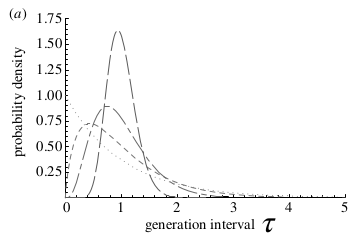
\includegraphics[width=0.8\textwidth]{../lessons/image/21/image07a.png}  \label{fig:21_07a} }
\end{minipage}
\begin{minipage}[]{0.5\linewidth}
\centering
\subfloat[][]{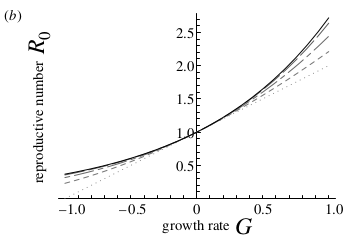
\includegraphics[width=0.8\textwidth]{../lessons/image/21/image07b.png}  \label{fig:21_07b} }
\end{minipage}
\caption{\label{fig:21_07} Different distributions to of generation times (\ref{fig:21_07a}) lead to different $R_0$ once we observe an exponential growth $G$ (\ref{fig:21_07b}).}
\end{figure}

Whereas, if we consider a \textbf{Delta Distribution}, i.e. a well peaked distribution with no variance at all, its transform is:
\begin{equation*}
    w(\tau) = \delta(T_c) \implies R_0 = e^{GT_c}
\end{equation*}
that sets an \textbf{Upper bound} of $R_0$. This is the case where the infection duration is more or less equal for everybody.

In other words, adding some variability onto a fixed $\expval{T_c}$ generation time, a given $R_0$ will correspond to higher $G$. This can be formalized thanks to \textbf{Jensen's inequality}: the average of transformed stochastic variables is at least equal to the transformed average of those variables when the transformation is \textit{convex}:
\begin{equation}
    \int_0^\infty e^{z\tau} w(\tau) d\tau \geqslant e^{z\int_0^\infty \tau w(\tau) d\tau} \implies \mathcal{M}_{w(\tau)}(z) \geqslant e^{z T_c} \implies R_0 \leqslant e^{GT_c}
\end{equation}

Recalling that $\tau$ is distributed according to some distribution $w(\tau)$, we assume that $\tau$ is the sum of two stochastic variables:
\begin{equation*}
    \tau = \tau_E + \tau_I
\end{equation*}
where $\tau_E$ is distributed according to $g(\tau_E)$ and $\tau_I$ follows another distribution, namely $h(\tau_I)$. One can prove that the generation times distribution $w(\tau)$ can be rewritten as the \textit{convolution} between $g$ and $h$:
\begin{equation}
    w(\tau) = g(\tau_E)*h(\tau_I)
\end{equation}
and, its Laplace transform is:
\begin{equation}
    \mathcal{M}_{w(\tau)} = \mathcal{M}_{g(\tau_E)} \times \mathcal{M}_{h(\tau_I)}
\end{equation}

This can turn out to be useful if we want to add some complexity to our model\footnote{What we observe in reality is that infectivity continuously evolves throughout time: sometimes it is less and sometimes is high. We can simplify and divide this behavior into two discrete stages: Exposed and Infected.} and consider the generation time as the sum of a \textbf{latent period}, during which \textit{no infections} can be generated and that distributes as $g(\tau_E)$, and a second term that is an \textbf{infection period} $\tau_I$ where infections can be generated and distributes as $h(\tau_I)$. For instance, let as assume that $\tau_E \sim Exp(\varepsilon)$ $\tau_I \sim Exp(\mu)$. The basic reproductive ratio is defined as $R_0 = \frac{1}{\mathcal{M(-G)}}$:
let us compute it analytically. We know that:
\begin{equation}
    \frac{1}{R_0} = \mathcal{M}(-G) = \int_{0}^{\infty} e^{-G \tau} \omega (\tau) d\tau
\end{equation}
Given $ g(\tau_E) = \varepsilon e^{-\varepsilon \tau_E} $ and $ g(\tau_I) = \mu e^{-\mu \tau_I} $
\begin{align*}
 \mathcal{M}(-G) & = \mathcal{M}_{g(\tau_E)} \cross \mathcal{M}_{h(\tau_I)} = \int_{0}^{\infty} e^{-G \tau_E} g(\tau_E) d\tau_E  \cross \int_{0}^{\infty} e^{-G \tau_I} g(\tau_I) d\tau_I\\
&= \int_{0}^{\infty} e^{-G \tau_E} \varepsilon e^{-\varepsilon \tau_E} d\tau_E \cross \int_{0}^{\infty} e^{-G \tau_I} \mu e^{-\mu \tau_I} d\tau_I\\
&= \varepsilon\int_{0}^{\infty} e^{-(G+\varepsilon) \tau_E} d\tau_E \cross \mu \int_{0}^{\infty} e^{-(G+\mu) \tau_I} d\tau_I\\
&= \frac{\varepsilon}{G+\varepsilon} \cross \frac{\mu}{G+\mu} = \frac{1}{R_0}
\end{align*}
The \textbf{basic reproductive ratio}:
\begin{align}
    {R_0}= \Big(1+\frac{G}{\varepsilon} \Big) \cdot \Big(1+\frac{G}{\mu} \Big) = 1+\frac{G}{\varepsilon}+\frac{G}{\mu}+\frac{G^2}{\varepsilon\cdot\mu} \cong 1+G(\varepsilon^{-1} + \mu^{-1})
\end{align}
One should note that we have exactly got back to the result of the \textbf{SEIR} model.


One should note however that if we observe an \textbf{exponential growth}, we cannot conclude \textit{anything} on the \textit{Basic Reproductive Ratio} $R_0$, since we need both average and variance information of \textbf{generation time distribution} as well: this indeed helps to interpret the exponential growth (Fig. \ref{fig:21_07b}).

\textbf{In practice}, when we have an \textbf{incidence time series} $\{ y_t \}$ we need to:
\begin{itemize}
    \item \textit{Define a time window} where the \textbf{growth} is \textbf{exponential}.
    \item We make a \textbf{Poisson regression} of the incidence points, assuming that our process is Poisson and with expected value:
    \begin{equation*}
        \log\ (\mathbb{E}(y_t|t)) = \alpha_0 + Gt
    \end{equation*}
    \item We estimate through the \textit{likelihood} both \textbf{initial conditions} and the \textbf{exponential growth}.
    \begin{equation*}
        \mathcal{L}(\alpha_0, G|\{y_t\}) = \prod_{t=0}^{t_M}\frac{e^{y_t(\alpha_0 + Gt)}e^{-e^{\alpha_0 + Gt}}}{y_t !}
    \end{equation*}
    Initial conditions are fundamental, since we need them to properly understand and interpret $G$. Even though we want to infer a single parameter and $\alpha_0$ has no specific meaning taken by itself, those are needed.
\end{itemize}

Clearly, the proper distribution of generation times is difficult to obtain analytically; therefore, we use only available information on the generation time distribution and make some assumptions in order to compute $R_0$.
Many times the only information we have is its \textit{average} $T_c$ and \textit{dispersion} $\sigma$, hence we can exploit the \textbf{Gaussian approximation}:
\begin{equation*}
    R_0 \simeq e^{GT_c-(1/2)G^2 \sigma^2}
\end{equation*}
However, often the \textbf{distribution of serial intervals} is used as a \textit{proxy} of the distribution of generation time.



\end{document}
